\documentclass[8pt]{article}
\usepackage[utf8]{inputenc}
\usepackage[spanish]{babel}

%Fuente (compilarlo en Latex.pdf normal porque va más rápido y luego
%y al final insertarlo en Arial) DA ERROR
%\usepackage{fontspec}
%\setmainfont{Arial}

%Estructura de la Página
\usepackage[left=2.54cm,right=2.54cm,top=2.54cm,bottom=2.54cm]{geometry}

%Páginas en horizontal


%Pies de página y encabezado
\usepackage{fancyhdr}

%Comentario párrafos
\usepackage{verbatim}

%Paquete arquitectura página
\pagestyle{fancy}
\fancyhf{}
\lhead{José Honrubia Blanco}
\rhead{Exámenes Ingeniería Térmica.}
\rfoot{\thepage}
\lfoot{Academia David Martínez}

%Interlineado
\renewcommand{\baselinestretch}{1}



%Paquete Matemático
\usepackage{amsmath}
\usepackage{amsfonts}
\usepackage{amssymb}
\usepackage{breqn}

%Paquete para el código
% Paquetes Listing

\usepackage{listings}
\usepackage{xcolor}

%Settings 

\definecolor{codegreen}{rgb}{0,0.6,0}
\definecolor{codegray}{rgb}{0.5,0.5,0.5}
\definecolor{codepurple}{rgb}{0.58,0,0.82}
\definecolor{backcolour}{rgb}{0.95,0.95,0.92}


\lstdefinestyle{mystyle}{
 backgroundcolor=\color{backcolour},   
 commentstyle=\color{codegreen},
 keywordstyle=\color{magenta},
 numberstyle=\tiny\color{codegray},
 stringstyle=\color{codepurple},
 basicstyle=\ttfamily\footnotesize,
 breakatwhitespace=false,         
 breaklines=true,                 
 captionpos=b,                    
 keepspaces=true,                 
 numbers=left,                    
 numbersep=5pt,                  
 showspaces=false,                
 showstringspaces=false,
 showtabs=false,                  
 tabsize=2
}

\lstset{style=mystyle}
%Paquete Imágenes

\usepackage{graphicx}
\usepackage{subcaption}
\graphicspath{ {imagenes/} }



%Bibliografía
\usepackage[backend=bibtex]{biblatex}
\addbibresource{referencias.bib}

%Espacio entre párrafos
\setlength{\parskip}{0.05cm}
%Sangría
\setlength{\parindent}{0cm}




\title{Exámenes Ingeniería Térmica}
\author{José Honrubia Blanco }
\date{Noviembre 2022}

\begin{document}

\section{Examen Octubre 2022}
\subsection{TEORÍA}
\textbf{Pregunta 1}. (1 punto) Deduzca la ecuación de Mayer ($R = c _{p} - c _{v}$) a partir de la ecuación de los gases ideales y de la definición de entalpía.

\\ 
\textbf{Pregunta 2}. (1 punto) Un dispositivo cilindro pistón vertical contiene un gas a la presión de 100 kPa. La masa del pistón es de 5 kg y su diámetro 12 cm, determine: a) presión atmosférica que actúa sobre el gas (kPa). Se desea incrementar la presión del gas colocando un peso sobre el pistón, determine b) masa del peso que hay que colocar sobre el pistón para doblar la presión dentro del cilindro (kg)
Nota: tome $g= 9.81 \frac{m}{s ^{2}}$

\\
\textbf{Pregunta 3}. (1 punto)Un flujo de aire(gas perfecto, $c _{p} = 1.02 \frac{kJ}{kg K}$) entra a una tobera con una temperatura de 200 ºC, una presión de 300 kPa y una velocidad de $30 \frac{m}{s}$. La sección de entrada de la tobera es de $80 cm ^{2}$. A la salida la velocidad del aire es de 180 $\frac{m}{s}$ y la presión es de 100 kPa. Se puede considerar que la tobera es adiabática. Determine:
\begin{itemize}
    \item el flujo másico a través de la tobera (kg/s) y temperatura del aire a la salida (K)
    \item energía disponible perdida (kJ/kg) si $T _{0}= 293 K$ y $R _{aire} = 0.287 \frac{kJ}{kg K}$
\end{itemize}

\textbf{Pregunta 4}. (1 punto) Sobre una superficie gris y  opaca cuya temperatura es de 600 ºC incide la irradiación que se muestra en la figura. Si la emisividad de la superficie es 0.4. Calcular:
\begin{itemize}
    \item la transferencia de calor neta de la superficie ()$\frac{W}{m ^{2}}$)
    \item la reflectividad y la radiosidad ($\frac{W}{m ^{2}}$). Nota: $\sigma = 5.67 \cdot 10 ^{-8} \frac{W}{m ^{2}K}$ 
\end{itemize}
\begin{figure}[h!]
  \centering
  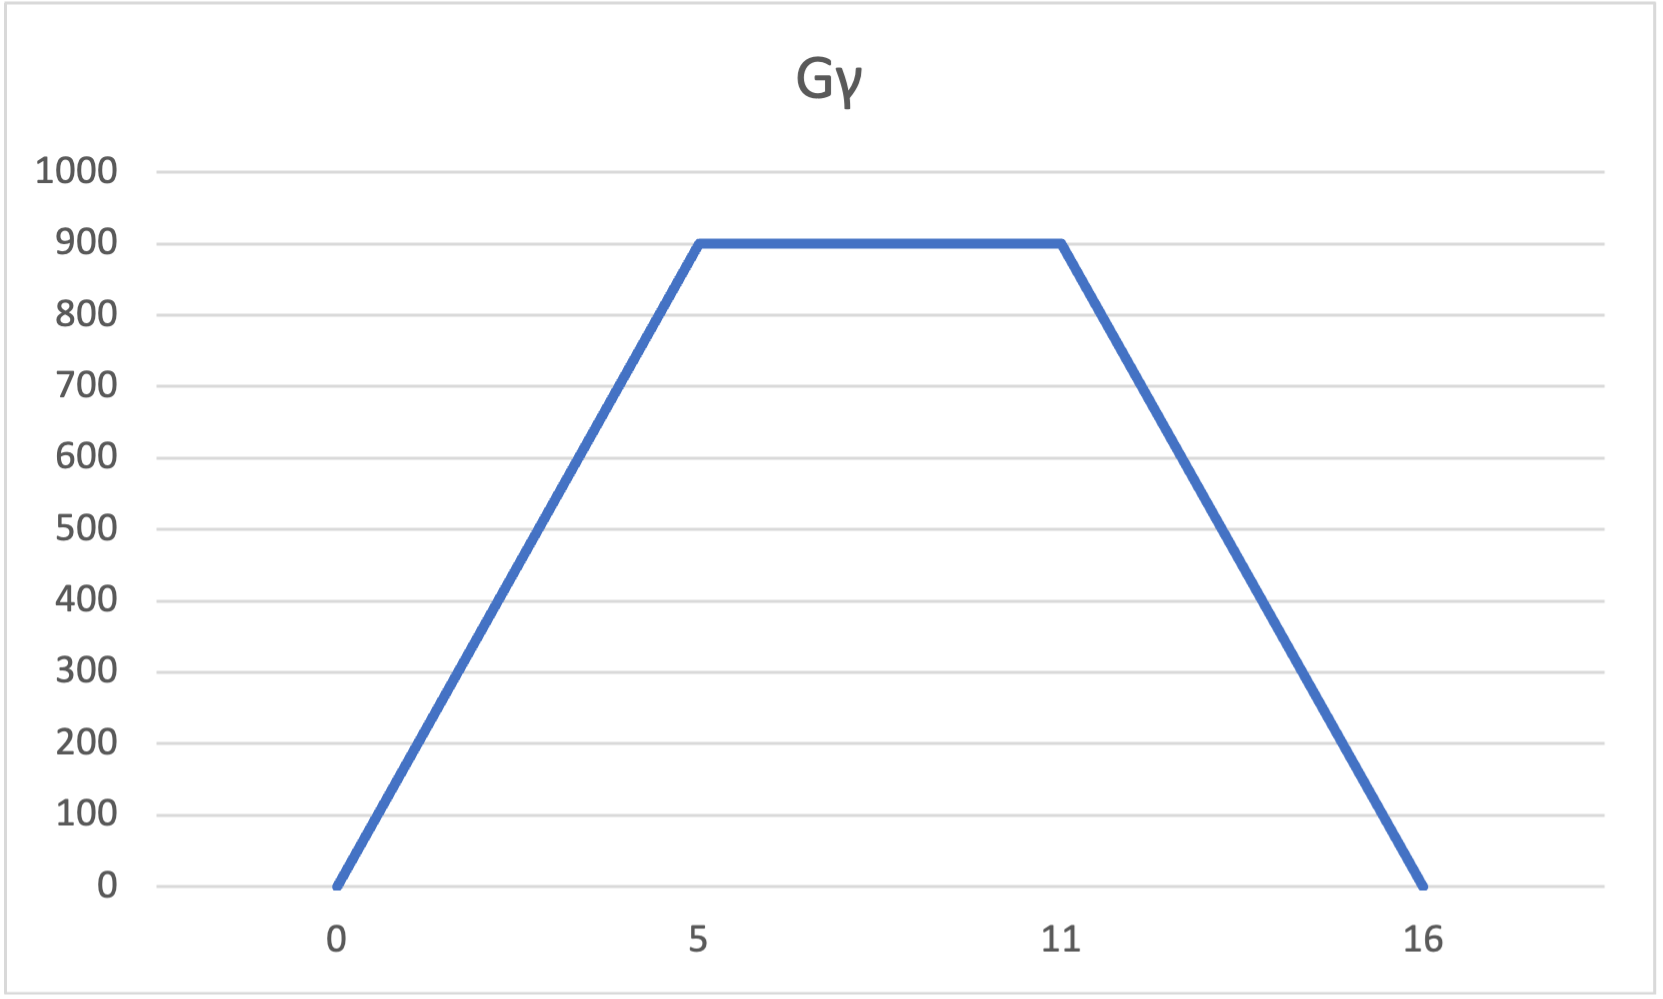
\includegraphics[width=0.3\linewidth]{imagen_1.png}
  \label{fig:}
\end{figure}

\\

\subsection{PROBLEMAS}
\textbf{Problema 1}. (\textbf{2 puntos}) Un tanque rígido contiene 2kmol de $N _{2}$ y 6 kmol de $CH _{4}$ y 12 MPa. Estime el volumen del tanque ($m ^{3}$) usando:
\begin{itemize}
    \item La ecuación de los gases ideales
    \item La regla de Kay
    \item La regla de Amagat
    \item Comente los resultados obtenidos
\end{itemize}

\textbf{Problema 2}. (\textbf{2 puntos}) Una central termica fucniona mediante el ciclo de Carnot. El vapor entra en la caldera en estado de líquido saturado (punto 1) a la presión de 40 bar y sale de ella en estado de vapor saturado (punto 2). Tras expandirse en la turbina, leega al condensador que está a 0.1 bar. Determine:
\begin{itemize}
    \item Diagrama T-s del ciclo termodinámico y T (ºC), P (bar), h (kJ/kg) y s (kJ/kg K)
    \item Rendimiento térmico del ciclo
    \item Variación de exergía del agua al pasar por la caldera (kJ/kg) despreciando la energía potencial y cinética y considerando la temperatura ambiente 300K
    \item ¿qué inconvenientes conlleva expandir en la zona de vapor húmedo?¿ qué otros inconvenientes presenta el ciclo de Carnot y cómo se modificia este dcilo para dar lugar a un ciclo Rankine?
\end{itemize}

\textbf{Problema 3}. (\textbf{2 puntos}) Un horno doméstico cocina con aire a una temperatura de 280 ºC. La temperatura interior del vidrio (pyrex) de la puerta de 1 cm de espesor es de 240 ºC y la exterior de 200 ºC. El vidrio tiene una conductividad térmica de $1.4 \frac{W}{m K}$ y una emisividad superficial del $0.7$. Teniendo en cuenta que la temperatura del ambiente es de 20 ºC. ¿Cuánto valen los coeficientes de transferencia de calor por convección libre al aire contigua a la superficie interior y exterior del vidrio?
Hipótesis: Condiión de estado estable. Trnsferencia de calor unidimensional por conducción a través del vidrio. Superficie gris $\epsilon = \alpha$.


\end{document}